\documentclass[spanish]{article}
\usepackage{graphicx}
\usepackage{ragged2e}
\usepackage{geometry}
\usepackage{float}
\usepackage{hyperref}
\usepackage[table,xcdraw]{xcolor}
\usepackage[ruled,vlined]{algorithm2e}
\title {Práctica  6: Algoritmos Greedy. Programacíon Dínamica.}
\graphicspath{{../img/}}
\addtolength{\textheight}{1.5in} 
\begin{document}
	\centerline{
\includegraphics[width=450px,height=100px]{header}}
	\centerline{Analisis de algoritmos, Sem: 2021-1, 3CV1,Práctica  6: Algoritmos Greedy. Programacíon Dínamica., 18/12/2020}
	\centering{\huge{Práctica  6: Algoritmos Greedy. Programacíon Dínamica}}
	\centerline{\newline{\textbf{Payán Téllez René}}}
	\newline{\textit{rpayant1500@alumno.ipn.mx}}
	\bigskip
	\justify
	\textbf{Resumen:}	
	En esta practica se analizaran 2 algoritmos que pertenecen a la programacion dinamica, la secuencia de fibonacci (por ambos caminos) y el segundo, el algoritmo "mochila 0-1"\\
	\textbf{Palabras clave:}
	DP, knapsack, Fibonacci, STL, C/C++
	\section{Introduccion}
	La programacion dinamica es una herramienta extremadamente poderosa para resolver problemas, principalmente aquellos con la premisa de "Cuantas formas hay de...", "Cual es el minimo/maximo de....", "Es posible....", ya que su premisa principal es generar todas las posibilidades dentro del problema, y analizar que casos se translapan, entonces a estos responderlos de forma rapida puesto que ya habian sido calculados. Si no se tiene cuidado esta poderosa herramienta puede resultar contraproducente ya que consumira tanta memoria y tiempo como el programador haya establecido, por eso siempre es necesario analizar cual es la mejor forma de resolver un problema de esta naturaleza. Por otra parte los algoritmos voraces son opuestos a las DP's, ya que no consideran los translapes, ni ven hacia atras, solo toman lo que tienen y reducen el tamaño de los datos hasta resolver el problema, son extremadamente rapidos de programar y en la ejecucion, sin mencionar que son altamente efectivos aunque no garantizen la mejor solución, por ello un buen programador debe ser capaz de implementar ambas herramientas y de determinar cual se adapta mejor a sus necesidades. En esta practica realizaremos 2 algoritmos de programacion dinamica, y con uno de ellos contrarrestaremos un ejemplo clasico de un algoritmo voraz (la mochila fraccionaria) con su contra parte "mochila 01". Tambien probaremos lo util de la memorizacion al reducir significativamente el tiempo de ejecucion al encontrar el n-simo termino de la sucesion de fibonacci.
	\section{Conceptos Basicos}
	\subsection{Algoritmo}
	La palabra algoritmo proviene del sobrenombre de un matemático árabe del siglo IX, Al-Khwarizmi, que fue reconocido por enunciar paso a paso las reglas para las operaciones matemáticas básicas con decimales (suma, resta, multiplicación y división).	
	Vemos definición de algoritmo como un grupo de órdenes consecutivas que presentan una solución a un problema o tarea. Algunos ejemplos de algoritmos los podemos encontrar en las matemáticas (como el algoritmo para resolver una multiplicación) y en los manuales de usuario de un aparato (como una lavadora o una impresora).	
	Sin embargo, hoy en día se relaciona la palabra algoritmo con el mundo de la informática, más concretamente en la programación; los conocidos como algoritmos informáticos.[1]	
	\subsection{Complejidad algoritmica}
	Así que, por su naturaleza, un problema tiene la capacidad de ser solucionado por uno o varios métodos, pero si bien es importante llegar a la respuesta, más importante es evaluar su viabilidad. Siempre que se analiza y evalúa adecuadamente la efectividad de una solución, disminuye drásticamente el costo que representa su producción y mantenimiento, pues los recursos que se invierten posteriormente en codificación, pruebas y revisión es mucho menor siempre (como el tiempo, dinero y talento humano).	
	Entrando en materia, la complejidad algorítmica es una métrica teórica que nos ayuda a describir el comportamiento de un algoritmo en términos de tiempo de ejecución (tiempo que tarda un algoritmo en resolver un problema) y memoria requerida (cantidad de memoria necesaria para procesar las instrucciones que solucionan dicho problema). Esto nos ayuda a comparar entre la efectividad de un algoritmo y otro, y decidir cuál es el que nos conviene implementar.[2]
	\subsection{Algoritmos Greedy o glotones}	
	Un algoritmo Greedy o gloton es un algoritmo muy util para encontrar soluciones aproximadas e inclusive la mas optima a problemas complejos, ya que las entregan en muy corto tiempo. Se llaman Greedy porque siempre "comen lo que tienen a la mano", no garantizan encontrar la mejor solucion, pero si una aproximacion bastante buena.[3]
	Estas son sus caracteristicas principales:
	\begin{itemize}
		\item Se utilizan generalmente para resolver problemas deoptimización (obtener el máximo o el mínimo).
		\item Toman decisiones en función de la información que está disponible en cada momento. está disponible en cada momento.
		\item Una vez tomada la decisión, ésta no vuelve a replantearse en el futuro.
		\item Suelen ser rápidos y fáciles de implementar.
		\item No siempre garantizan alcanzar la solución óptima[4]
	\end{itemize}
	\subsection{Programacion Dinamica}
	La programacion dinamica es una tecnica de optimizacion realmente eficiente y versatil. Si bien fue desarrollada especialmente para la resolución de problemas en Procesos de Decisión en Múltiples Pasos, diferentes investigaciones han mostrado que las mismas ideas pueden utilizarse en otro tipo de problemas de matemática aplicada,e incluso pueden ser útiles en el planteo de algunas cuestiones teóricas.[5]
	Existen 2 enfoques principales:
	\begin{itemize}
		\item top-down (se inicia desde la raiz del problema hacia los sub problemas y el backtracking regresa el resultado)
		\item buttom-up (se inicia desde el subproblema mas pequeño y se ocupa para resolver el mas grande de forma iterativa)
	\end{itemize}
	\subsection{Algoritmo de Fibonacci con DP}
	Esta sucesión fue descrita por Fibonacci como la solución a un problema de cría de conejos: "Cierto hombre tiene una pareja de conejos juntos en un lugar cerrado y desea saber cuántos son creados a partir de este par en un año cuando, de acuerdo a su naturaleza, cada pareja necesita un mes para envejecer y cada mes posterior procrea otra pareja".[6]\\
	Resolucion por top-down (con memorizacion):\\	
	\begin{algorithm}[H]
		\KwData{Entrada: n (El limite a obtener de la secuencia de fibonacci), fibo[](arreglo con los valores memorizados)}
		\KwResult{Retorna el n-simo termino de la secuencia de fibonacci}
		\If{fibo[n] $!=-1$ }{
			return fibo[n]\;	
		}
		return fibo[n] = calcfibo(n-2)+calcfibo(n-1)\;
		\caption{calcfibo(n, fibo)}
	\end{algorithm}
	Resolucion por buttom-up:\\	
	\begin{algorithm}[H]
		\KwData{Entrada: n (El limite a obtener de la secuencia de fibonacci), fibo[](arreglo con los valores memorizados)}
		\KwResult{Retorna el n-simo termino de la secuencia de fibonacci}
		\If{$n\leq1$ }{
			return 1\;
		}\Else{
			fibo[0] = 0\;
			fibo[1] = 1\;
			\For{$i\gets 2$ \KwTo $n$}{
				fibo[i] = fibo[i-1] + fibo[i-2]\;
			}
		}
		return fibo[n]\;
		\caption{calcfibo(n, fibo)}
	\end{algorithm}			
	\subsection{Mochila 0-1}			
	Dados pesos y valor de n objetos, debemos poner estos en una mochila con una capacidad maxima "W". En otras palabras, dados 2 arreglos de enteros val[0,..,n-1] y wt[0,...,wt] los cuales representan valores y peso de los objetos respectivamente, posteriormente un entero "W", encontrar la maxima cantidad de objetos que podemos guardar dentro de la mochila. No puedes romperlos, solo tomarlos de forma entera o no hacerlo (propiedad 0-1).\\
	\begin{algorithm}[H]
		\KwData{Entrada: W (el peso maximo de la mochila), wt[1,...,n] (el peso de los objetos), val[1,...,n]  (el valor de los objetos)}
		\KwResult{Retorna g[0,...,n][0,...,W] una matriz con los valores calculados de la DP}
		\For{$c\gets 0\   \KwTo\   c\leq W$}{
			g[0,c] = 0\;
		}
		\For{$j\gets 0\   \KwTo\   j\leq n$}{
			g[j,0] = 0\;
		}
		\For{$j\gets 1\   \KwTo\   j\leq n$}{
			\For{$c\gets 1\   \KwTo\   c\leq W$}{
				\If{$c<wt[j]$}{
					g[j,c] = g[j-1,c]\;
				}\Else{
					\If{$g[j-1,c]\geq g[j-1,c-wt[j]] + val[j]$}{
						g[j,c] = g[j-1,c]\;
					}\Else{
						g[j,c] = g[j-1,c-wt[j]]+val[j]\;
					}
				}		
			}
		}
		return g\;
		\caption{mochila01(W, wt[1,...,n], val[1,...,n])}
	\end{algorithm}		
	\begin{algorithm}[H]
		\KwData{Entrada: j (la posicion sobre los objetos en la matriz), c (la posicion sobre el peso de la mochila), wt[1,...,n] (el peso de los objetos), val[1,...,n]  (el valor de los objetos),  g[0,...,n][0,...,W] (matriz calculada)}
		\KwResult{}
		\If{$j>0$}{
			\If{$c<wt[j]$}{
				test(j-1,c)\;			
			}\Else{
				\If{$g[j-1,c-wt[j]]+ val[j] > g[j-1,c]$}{
					test(j-1,c-wt[j])\;
					print("Guardar objeto ",j)\;
				}\Else{
					test(j-1,c)\;
				}
			}			
		}			
		\caption{test(j, W, wt[1,...,n], val[1,...,n], g[0,...,n][0,...,W])}
	\end{algorithm}		
	\section{Experimentacion y Resultados}
	\subsection{Implementar el algoritmo de Fibonacci por top-down y buttom-up.}
	Para poder analizar la complejidad de ambos acercamientos, se codificaron en el lenguaje de programacion C, se agregaron a las funciones de calcfibo un contador de operaciones para poder medir el total de las mismas. Para poder generar la grafica se implemento un ciclo que llama a la funcion calcFiboTopDown y calcFiboButtomUp con ($1\leq n\leq 46$) y al final se almaceno la complejidad de ambas funciones.\\
	\begin{figure}[H]
		\centering
		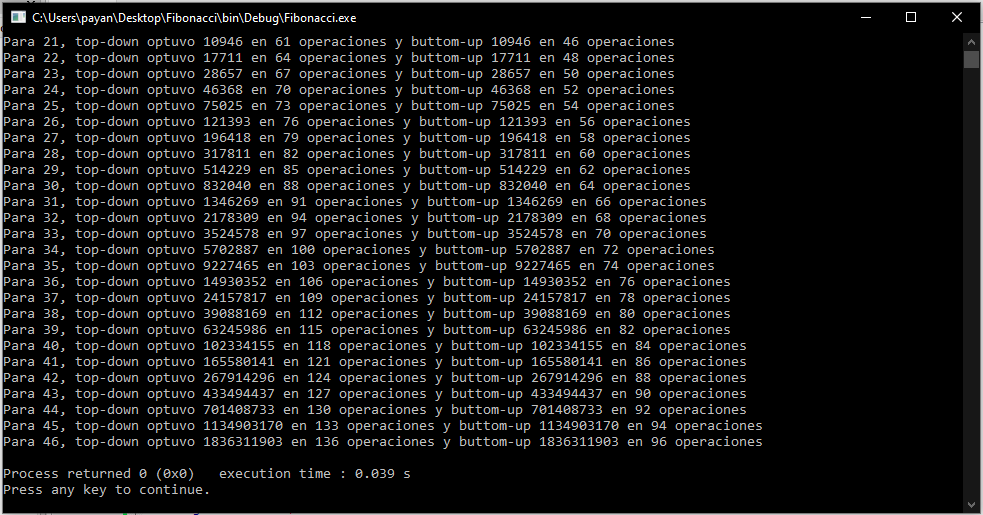
\includegraphics[width=400px,height=300px]{captura1}
		\caption{Ejecucion de ambas funciones}
	\end{figure}
	Una vez terminada la ejecucion se graficaron ambos resultados en las siguientes graficas.\\
	\begin{figure}[H]
		\centering
		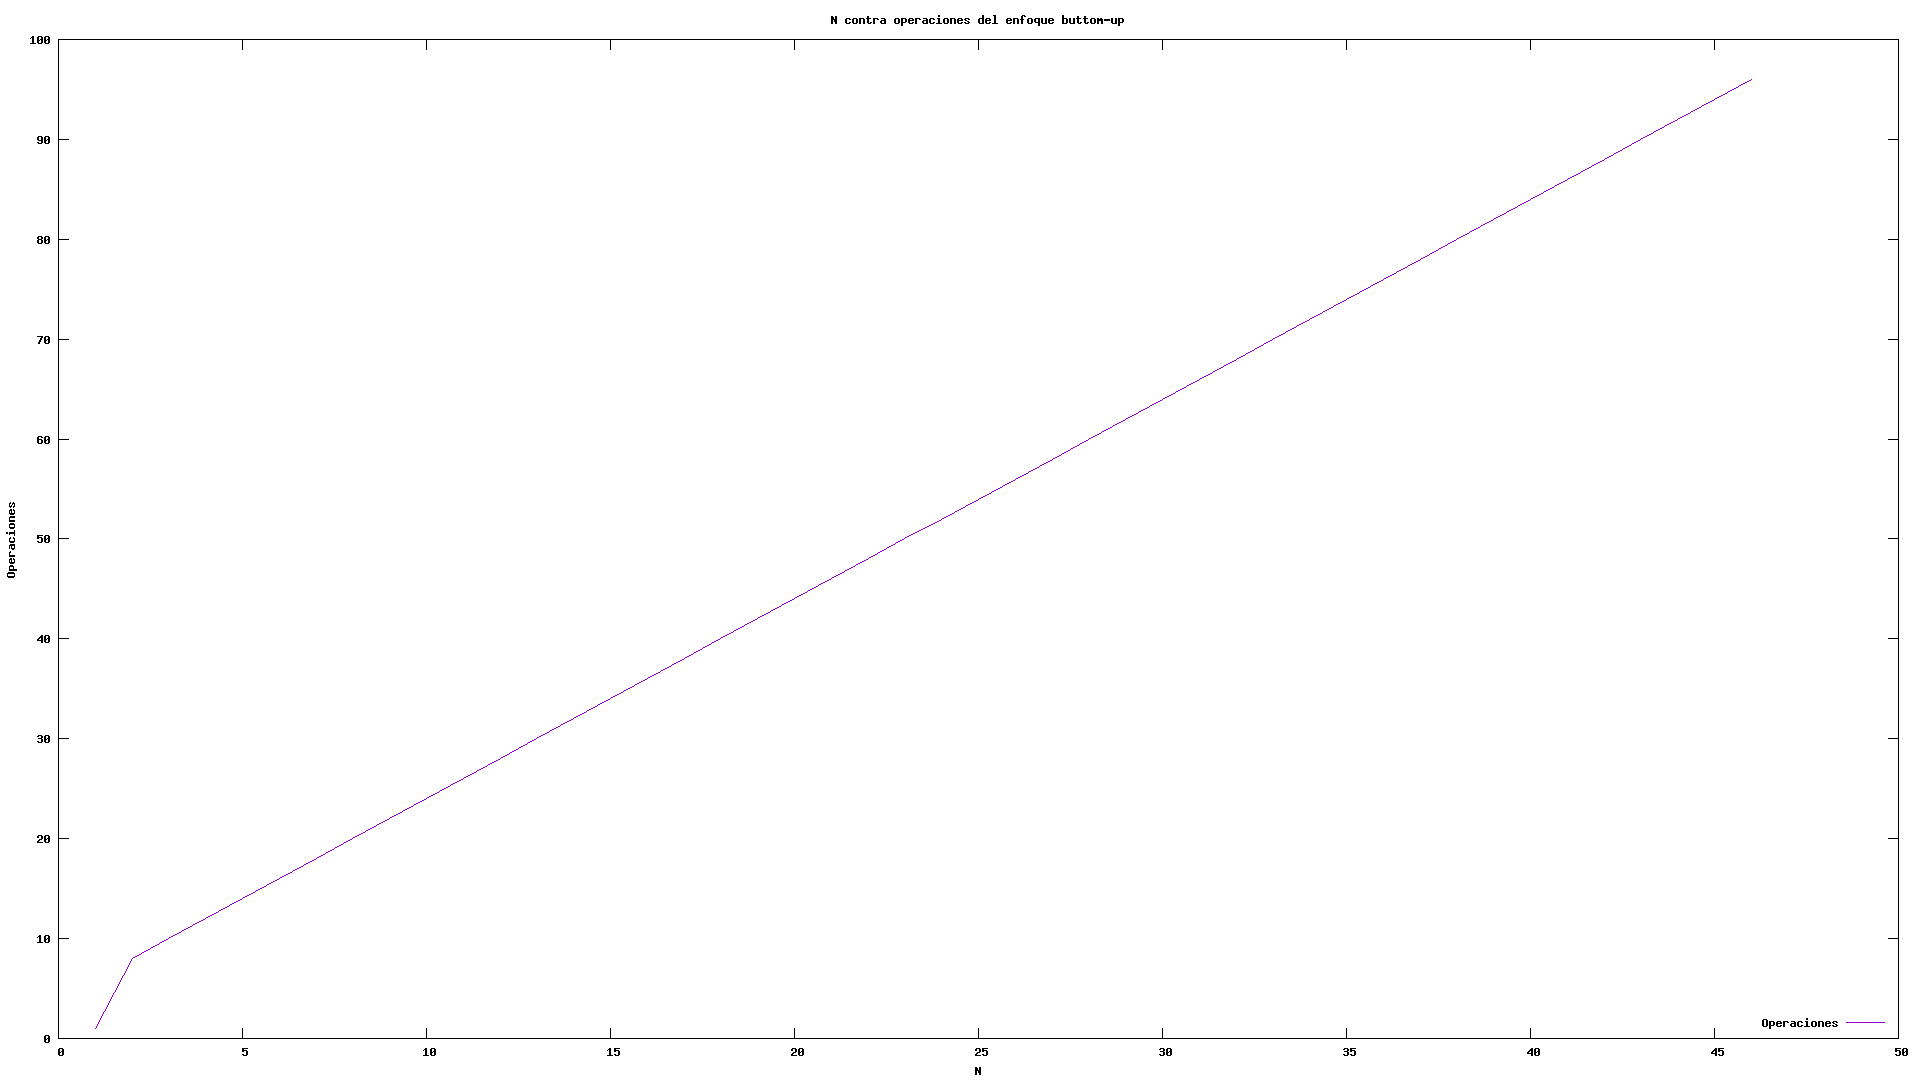
\includegraphics[width=400px,height=300px]{grafica1}
		\caption{N contra operaciones de buttom-up}
	\end{figure}
	\begin{figure}[H]
		\centering
		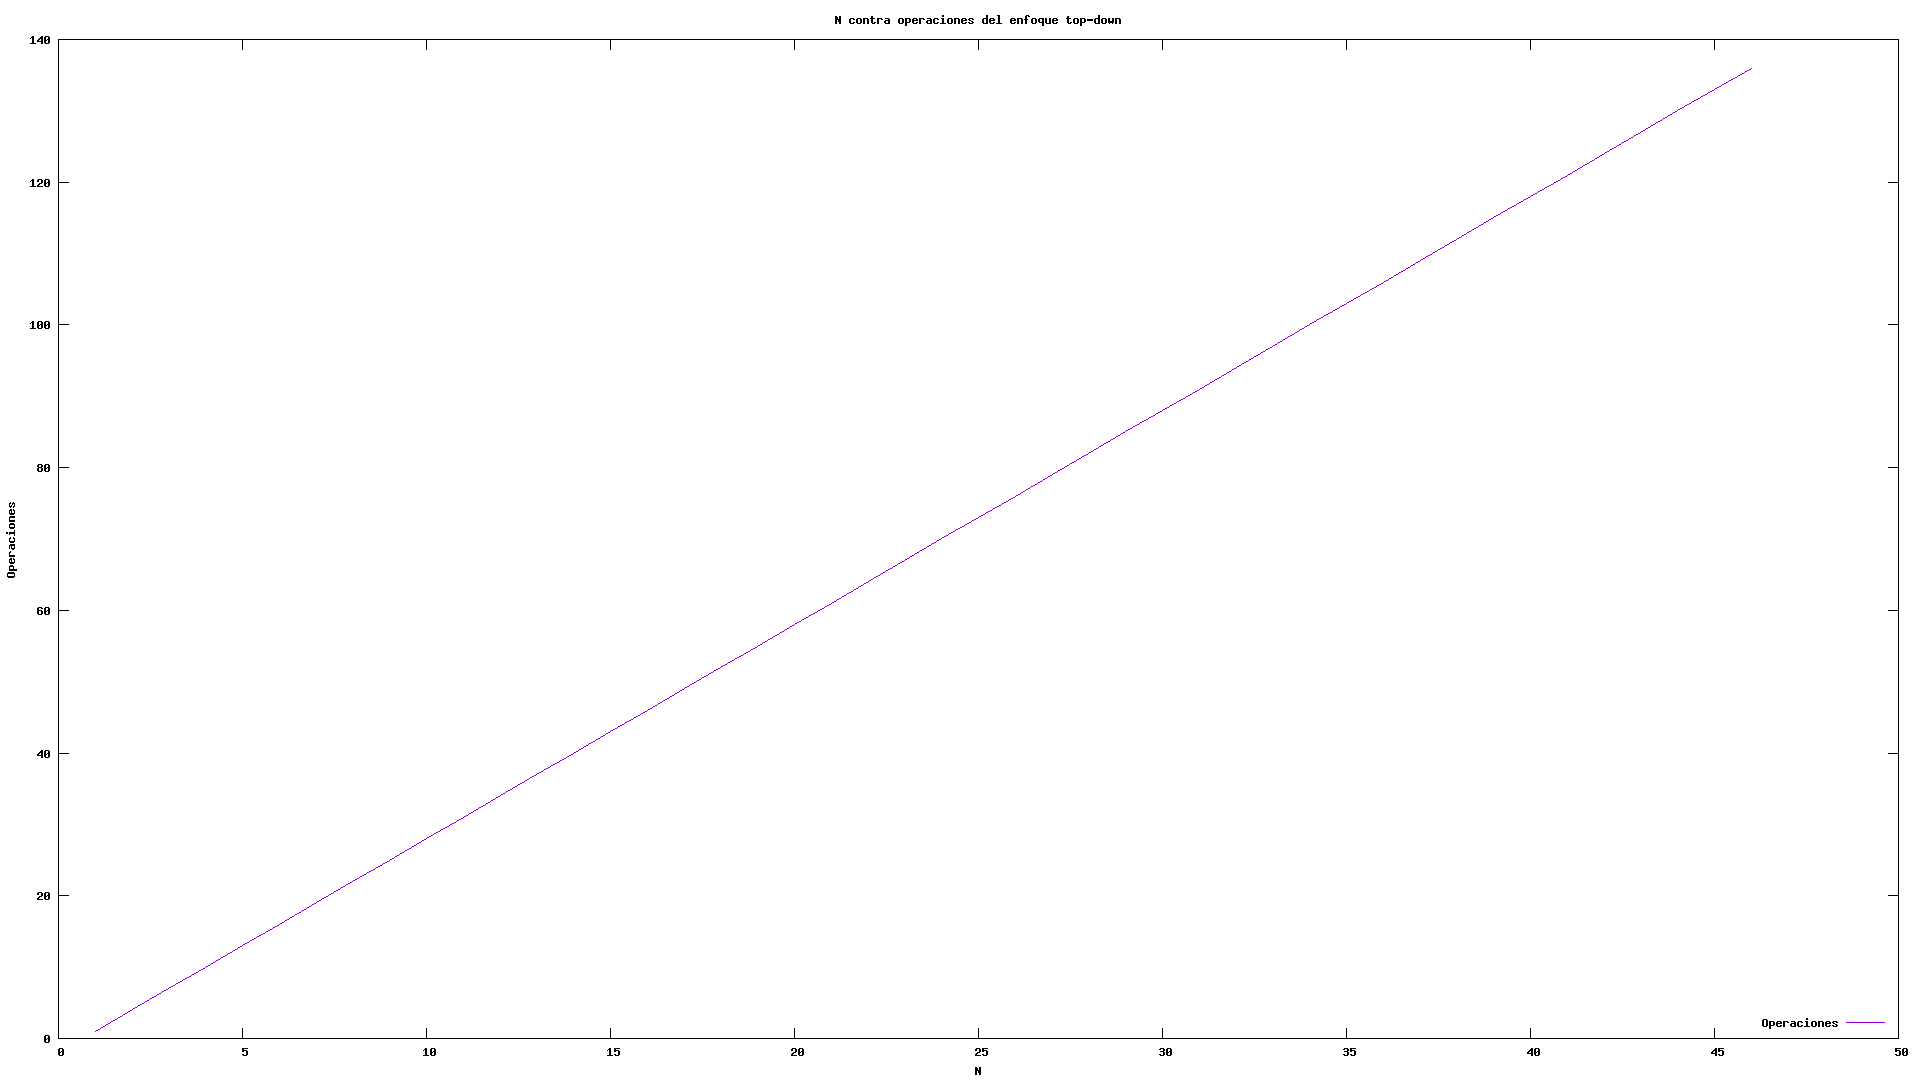
\includegraphics[width=400px,height=300px]{grafica2}
		\caption{N contra operaciones de top-down}
	\end{figure}
	\begin{figure}[H]
		\centering
		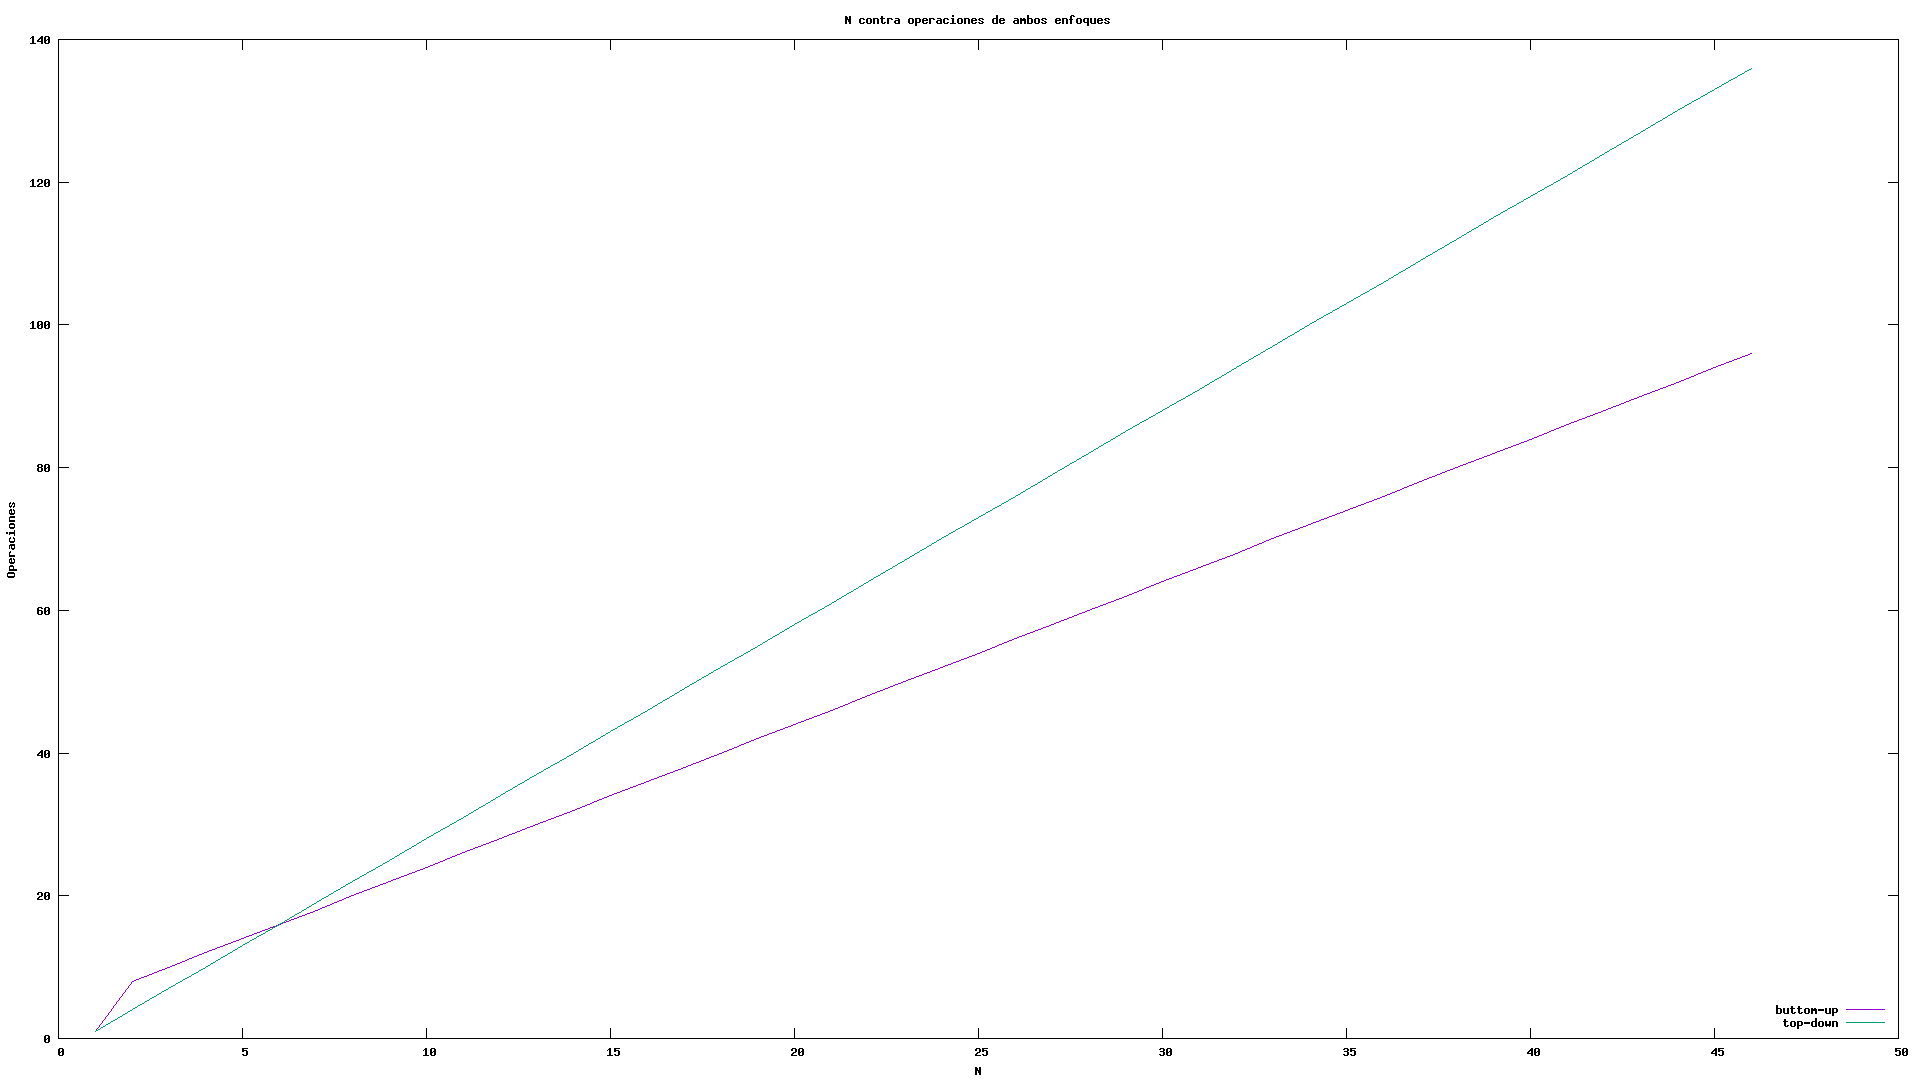
\includegraphics[width=400px,height=300px]{grafica3}
		\caption{N contra operaciones de ambas funciones}
	\end{figure}
	Ya con los resultados a posteriori, se realiza el calculo a priori de ambas funciones, primero se calcula la complejidad de buttom-up:\\
	\begin{center}
		\begin{table}[H]
			\begin{tabular}{|l|l|l|}
				\hline
				\rowcolor[HTML]{FFCC67} 
				Codigo                           & Costo & Veces ejecutado \\ \hline
				\textit{if(n<=1)}                    & $\O(1)$    & 1               \\ \hline
				\textit{\  \  return 1}                    & $\O(1)$    & 1               \\ \hline
				\textit{else}                    & $\O(1)$    & 1               \\ \hline
				\textit{\  \  fibo[0]=0}                    & $\O(1)$    & 1               \\ \hline
				\textit{\  \  fibo[1]=1}                    & $\O(1)$    & 1               \\ \hline				
				\textit{\  \  for(i=2;i$\leq$n;i++)} & $\O(n)$    & $n-1$             \\ \hline
				\textit{\  \  \  \  fibo[i] = fibo[i-1]+fibo[i-2]}                 & $\O(1)$    & $n-2$               \\ \hline
				\textit{return fibo[n]} & $\O(1)$    & $1$             \\ \hline				
			\end{tabular}
		\end{table}										
	\end{center}
	ahora si analizamos la funcion, lo que mas operaciones realiza es el ciclo desde 2 hasta n, es decir la funcion tiene orden de complejidad lineal.
	Como podemos ver y respaldados por las graficas (Figure 2 y Figure 4), la complejidad de esta funcion es $\O(n)$.\\
	Luego se realiza el analisis de complejidad de la implementacion via top-down:\\
	\begin{center}
		\begin{table}[H]
			\begin{tabular}{|l|l|l|}
				\hline
				\rowcolor[HTML]{FFCC67} 
				Codigo                           & Costo & Veces ejecutado \\ \hline
				\textit{if(fibo[n]$!=-1$)}                    & $\O(1)$    & 1               \\ \hline
				\textit{\  \  return fibo[n]}                    & $\O(1)$    & 1               \\ \hline
				\textit{else}                    & $\O(1)$    & 1               \\ \hline
				\textit{\  \  return fibo[n] = calcfibo(n-1)+calcfibo(n-2)}                    & $T(n-1)+T(n-2)$    & 1               \\ \hline 				
			\end{tabular}
		\end{table}										
	\end{center}
	Este calculo por su parte nos deja la siguiente ecuacion de recurrencia:\\
	\begin{equation}
		T(n)= \left\{ \begin{array}{lcc}
			0 &   si  & n = 0 \\
			1 &   si  & n = 1 \\
			T(n-1) +T(n-2) &  si &  n >= 2  \\
		\end{array}
		\right.
	\end{equation}
	con $T(0) = 0$ y $T(1) = 1$, podemos calcular la ecuacion de recurrencia de la siguiente forma:\\$		ax(n)+bx(n-1)+cx(n-2)=f(n)$, con a = 1, b = -1, c = -1, f(n) = 0\\
	como $f(n)=0$ podemos decir que es homogenea, por lo tanto la ecuacion caracteristica sería: $ar^2+br+c=0$\\
	calculando $r_1$ y $r_2$, obtenemos que $r_1=\frac{-1+\sqrt{5}}{2}$ y $r_2=\frac{-1-\sqrt{5}}{2}$, lo cual corresponde al caso 3
	1, por lo tanto $x(n)=\alpha(\frac{-1+\sqrt{5}}{2})^n+\beta(\frac{-1-\sqrt{5}}{2})^n$, sustituyendo cuando n = 0 y cuando n = 1, nos queda: $x(0) = 0 = \alpha(\frac{-1+\sqrt{5}}{2})^0 + \beta(\frac{-1-\sqrt{5}}{2})^0 = \alpha + \beta$ y $x(1) = 1 = \alpha(\frac{-1+\sqrt{5}}{2})^1 + \beta(\frac{-1-\sqrt{5}}{2})^1 = \alpha(\frac{-1+\sqrt{5}}{2}) + \beta(\frac{-1-\sqrt{5}}{2})$
	, resolviendo el sistema de ecuaciones, obtenemos que $\alpha=\frac{1}{\sqrt{5}}$ y $\beta=-\frac{1}{\sqrt{5}}$, quedando asi que $T(n) = n+2$ por lo tanto $T(n) = \frac{1}{\sqrt{5}}(\varphi^n + \hat{\varphi }^n)$, asi que $T(n)\in \theta(\varphi^n)$ consideremos que para el calculo de esta ecuacion de recurrencia no se considero la memorizacion de la DP, ya que no es predecible, se asumio el peor caso donde nada esta memorizado (cosa que no sucede de verdad), pero si miramos las graficas (Figure 2 y Figure 4) podemos ver que tiene una complejidad lineal (anque si superior al enfoque buttom-up).
	\subsection{Implementar el algoritmo de Mochila 0-1.} 
	Para poder analizar la complejidad a posteriori de este algorimo se implementaron las funciones "mochila01"y "test", luego se itero ($1\leq n\leq 2000$) elementos, pero determine que tambien el peso afectaba seriamente a la complejidad, asi que para este experimento, decidí dejarlo fijo en 500. Cada funcion tiene un contador por aparte como se podra apreciar en las capturas.
	\begin{figure}[H]
		\centering
		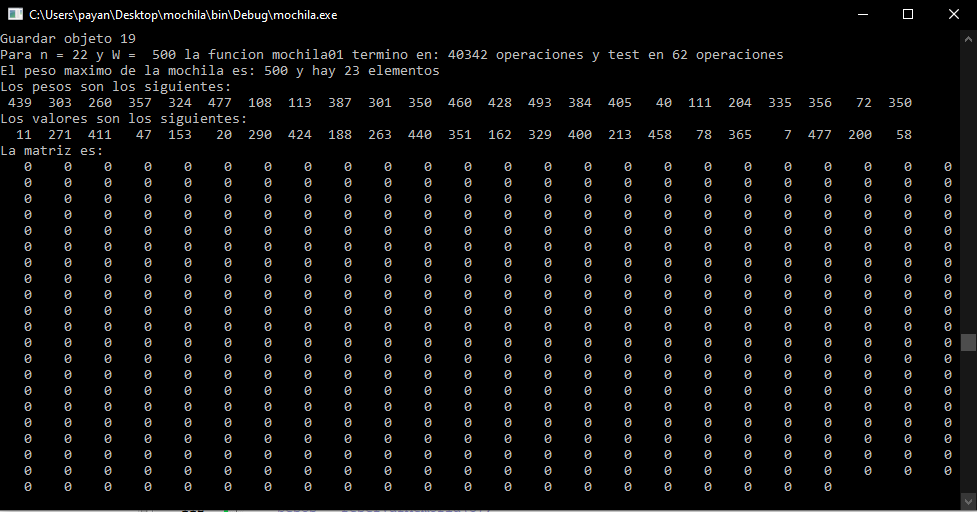
\includegraphics[width=400px,height=300px]{captura2}
		\caption{Ejecucion iterando sobre n}
	\end{figure}
	\begin{figure}[H]
		\centering
		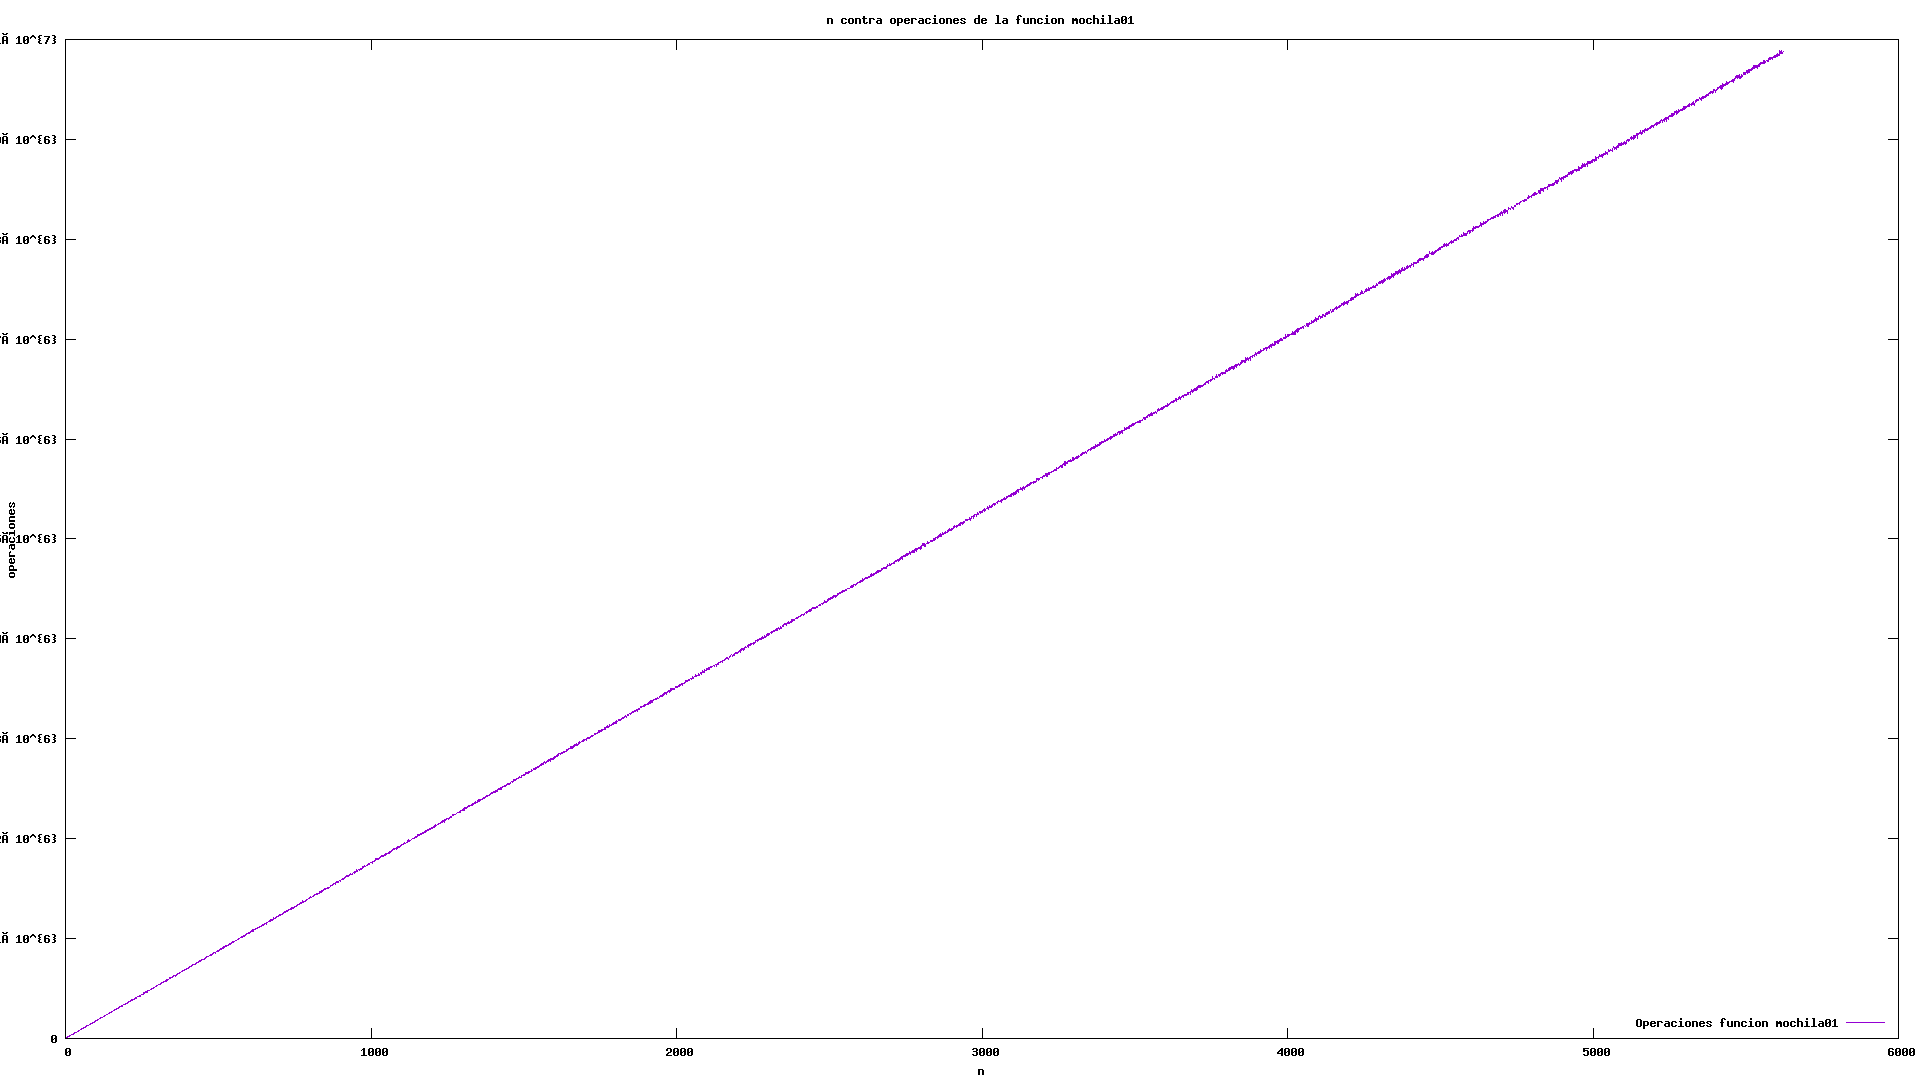
\includegraphics[width=400px,height=300px]{grafica4}
		\caption{n contra operaciones de la funcion mochila01}
	\end{figure}
	\begin{figure}[H]
		\centering
		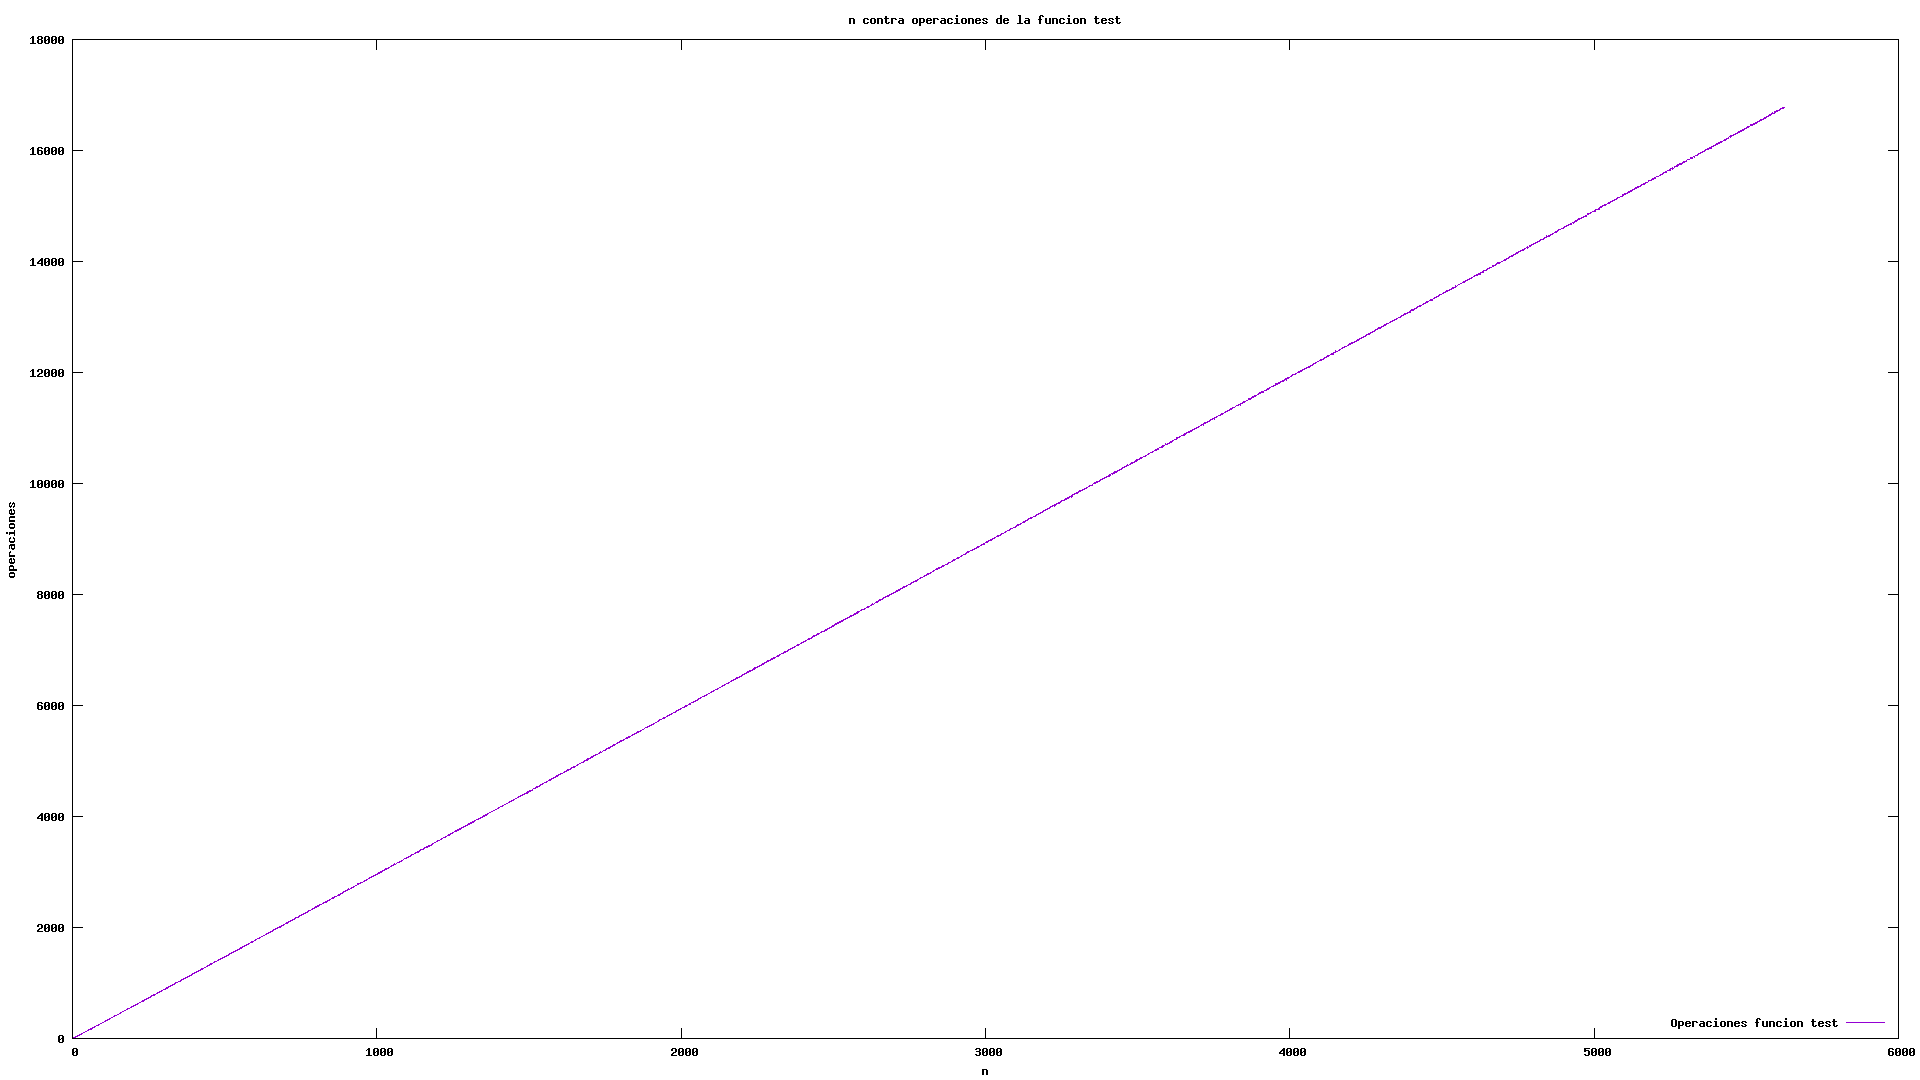
\includegraphics[width=400px,height=300px]{grafica5}
		\caption{n contra operaciones de la funcion test}
	\end{figure}
	\begin{figure}[H]
		\centering
		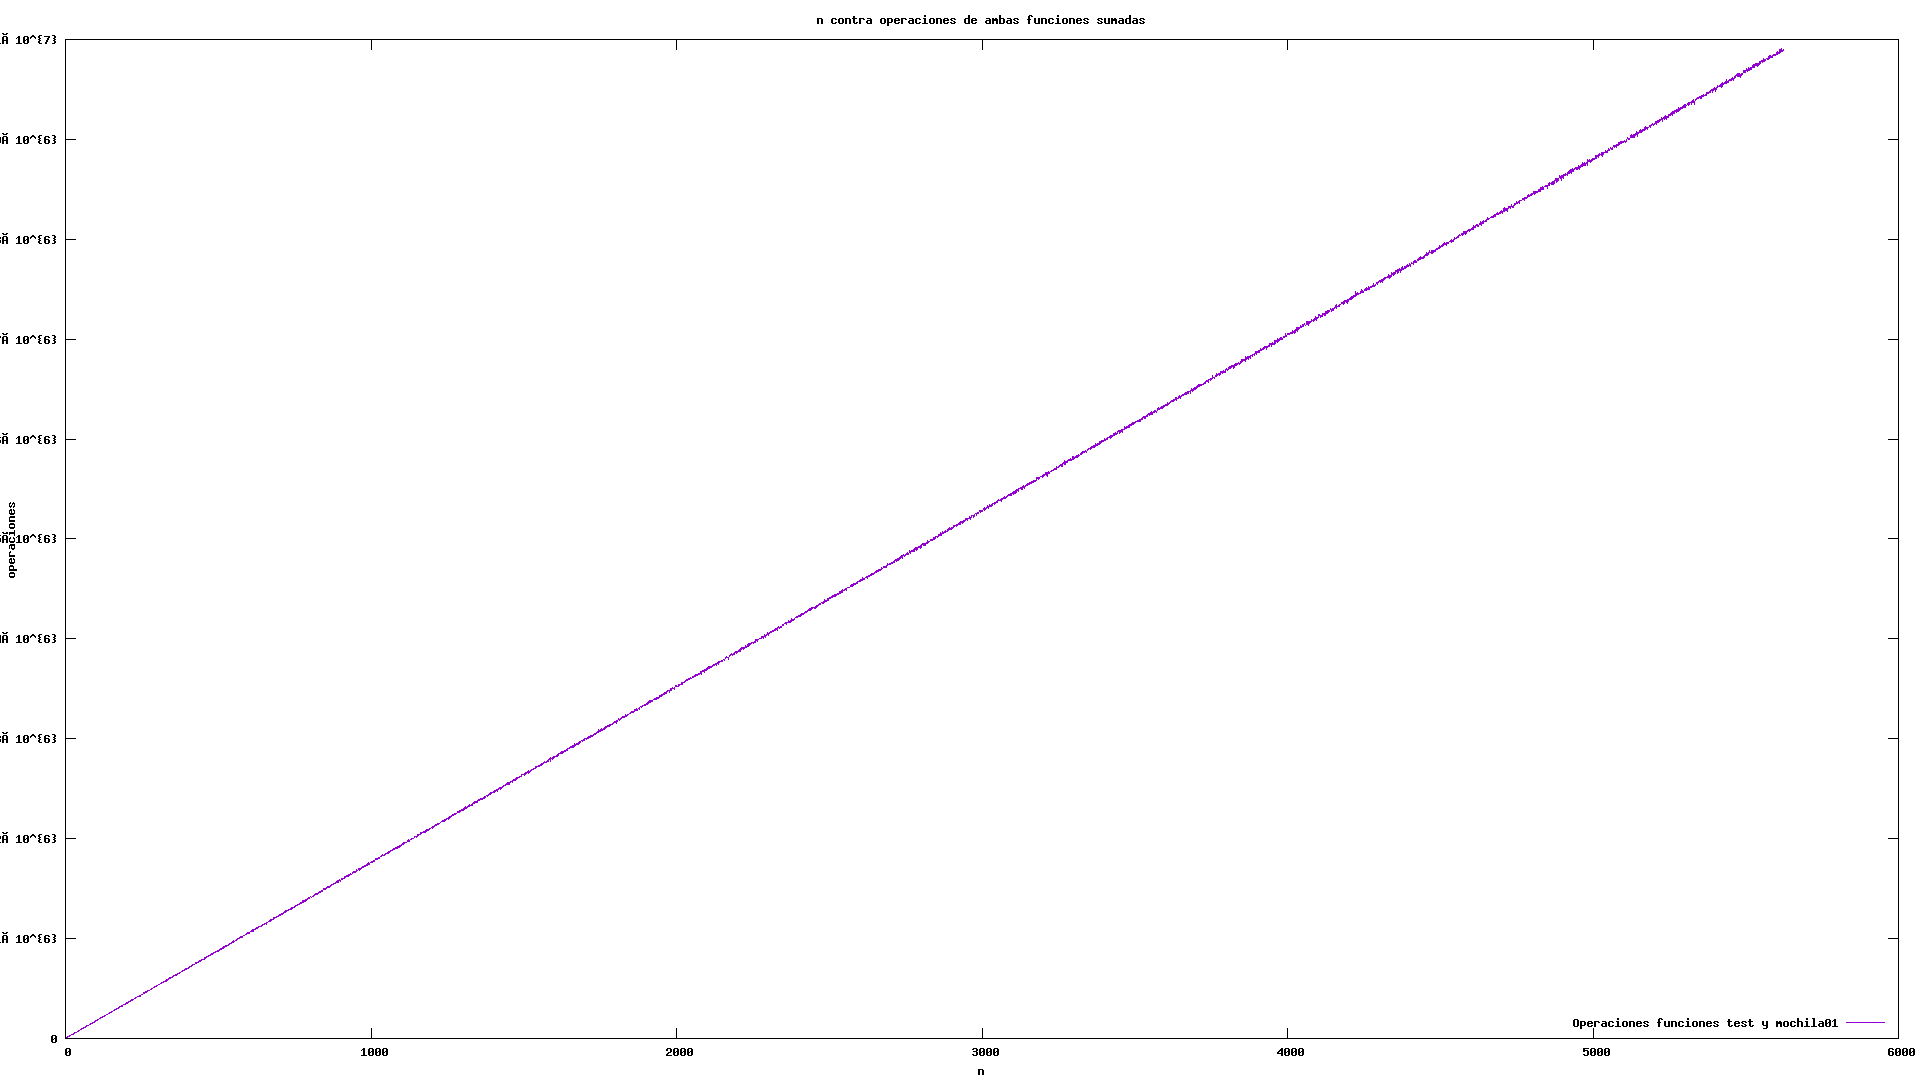
\includegraphics[width=400px,height=300px]{grafica6}
		\caption{n contra operaciones de ambas funciones sumadas}
	\end{figure}
	\begin{figure}[H]
		\centering
		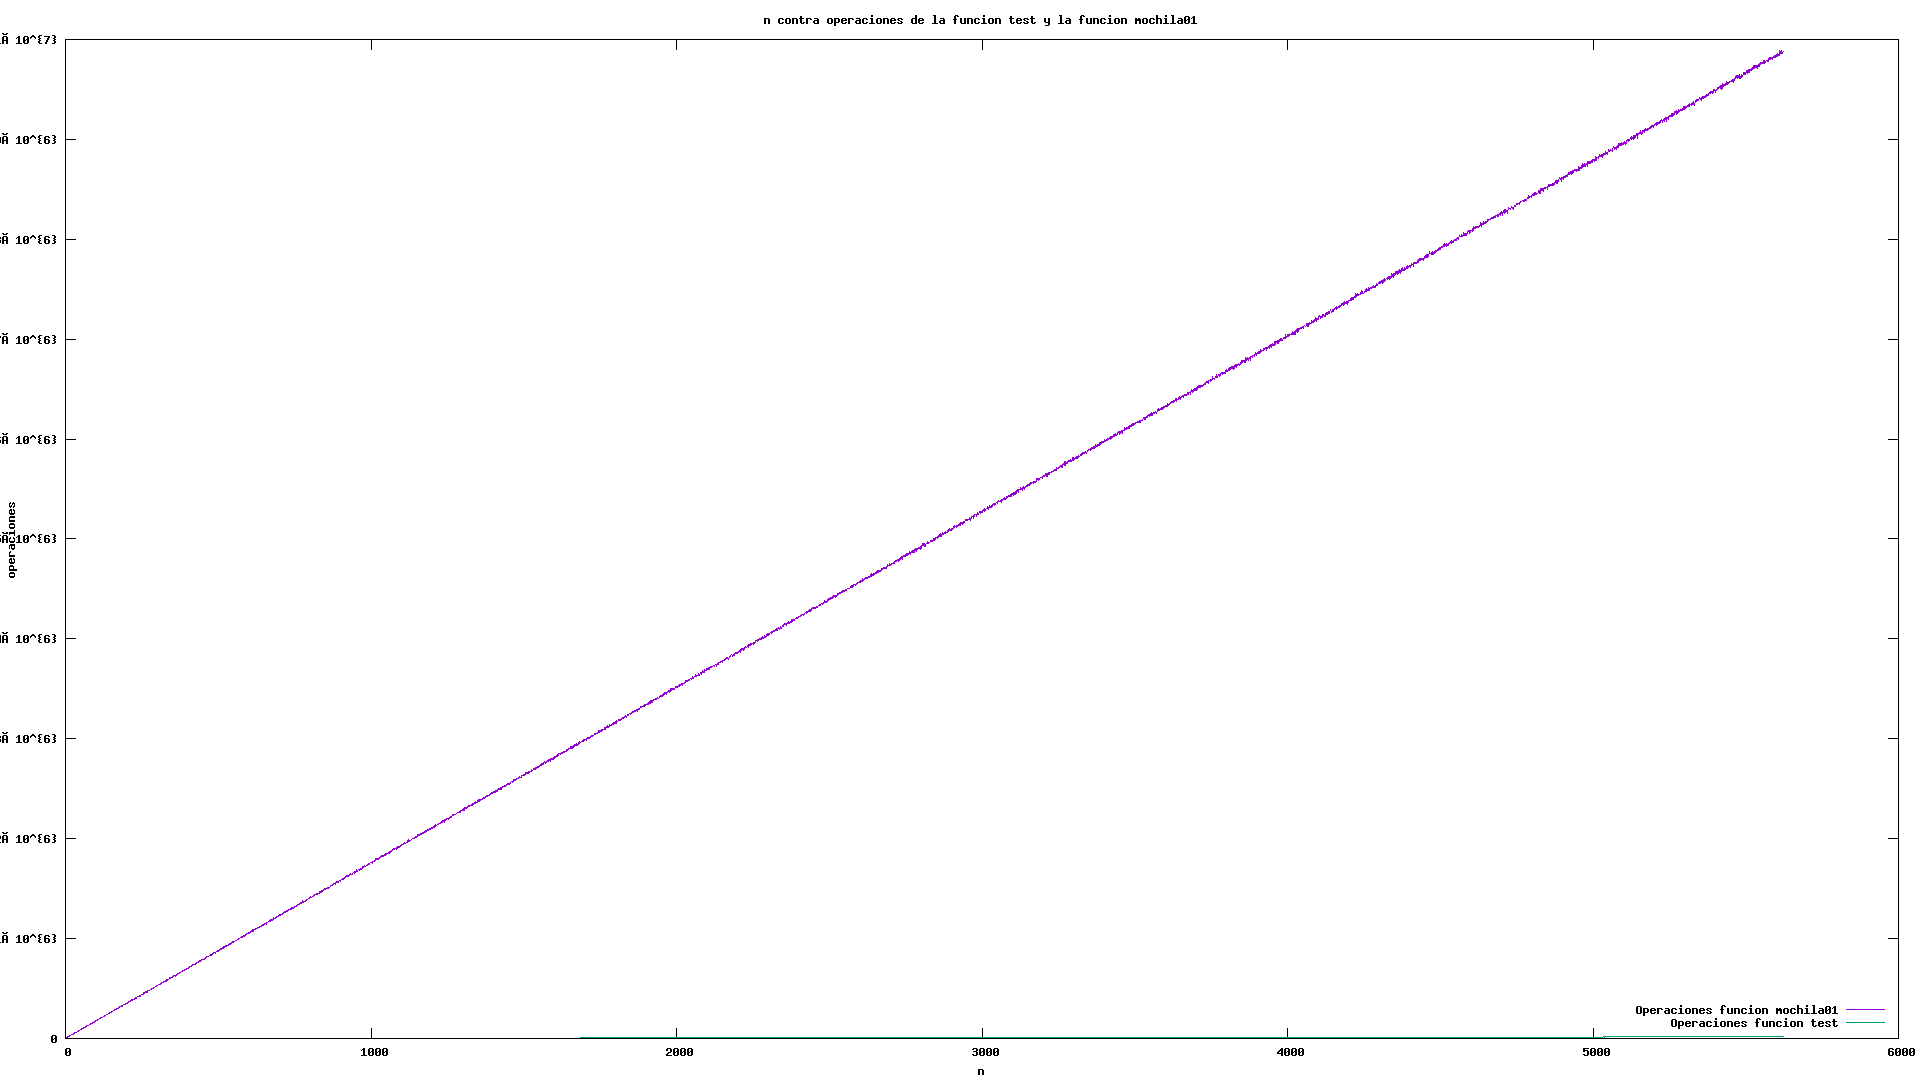
\includegraphics[width=400px,height=300px]{grafica7}
		\caption{n contra operaciones de la funcion test y la funcion mochila01}
	\end{figure}
	Una vez que se terminaron las pruebas a granel con n variable, se intercambio dicha regla, dejando n estatica en 500 y se itero sobre W en cambio.\\
	\begin{figure}[H]
		\centering
		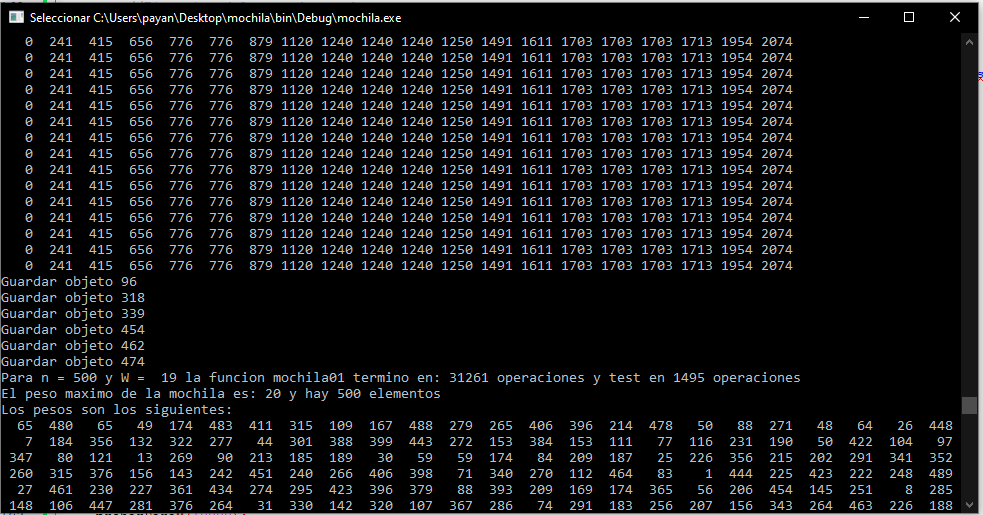
\includegraphics[width=400px,height=300px]{captura3}
		\caption{Ejecucion iterando sobre W}
	\end{figure}
	\begin{figure}[H]
		\centering
		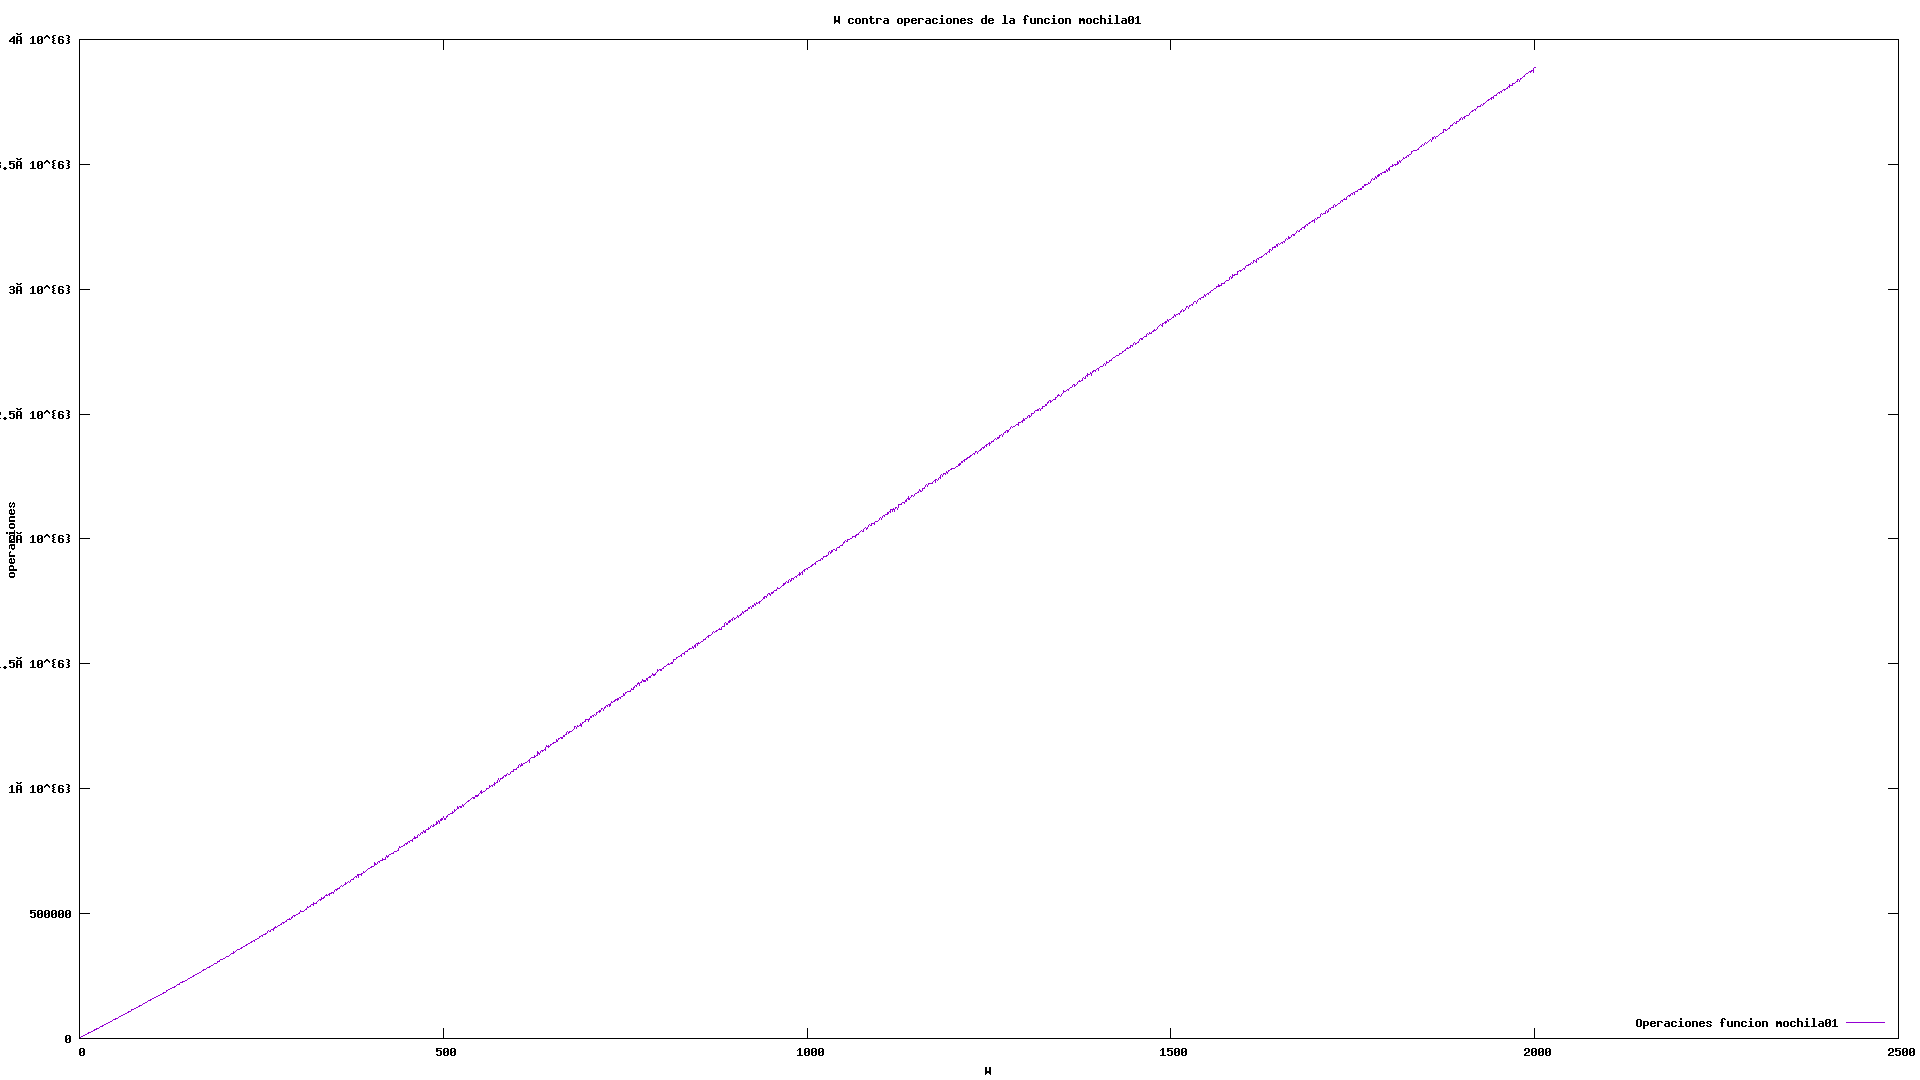
\includegraphics[width=400px,height=300px]{grafica8}
		\caption{W contra operaciones de la funcion mochila01}
	\end{figure}
	\begin{figure}[H]
		\centering
		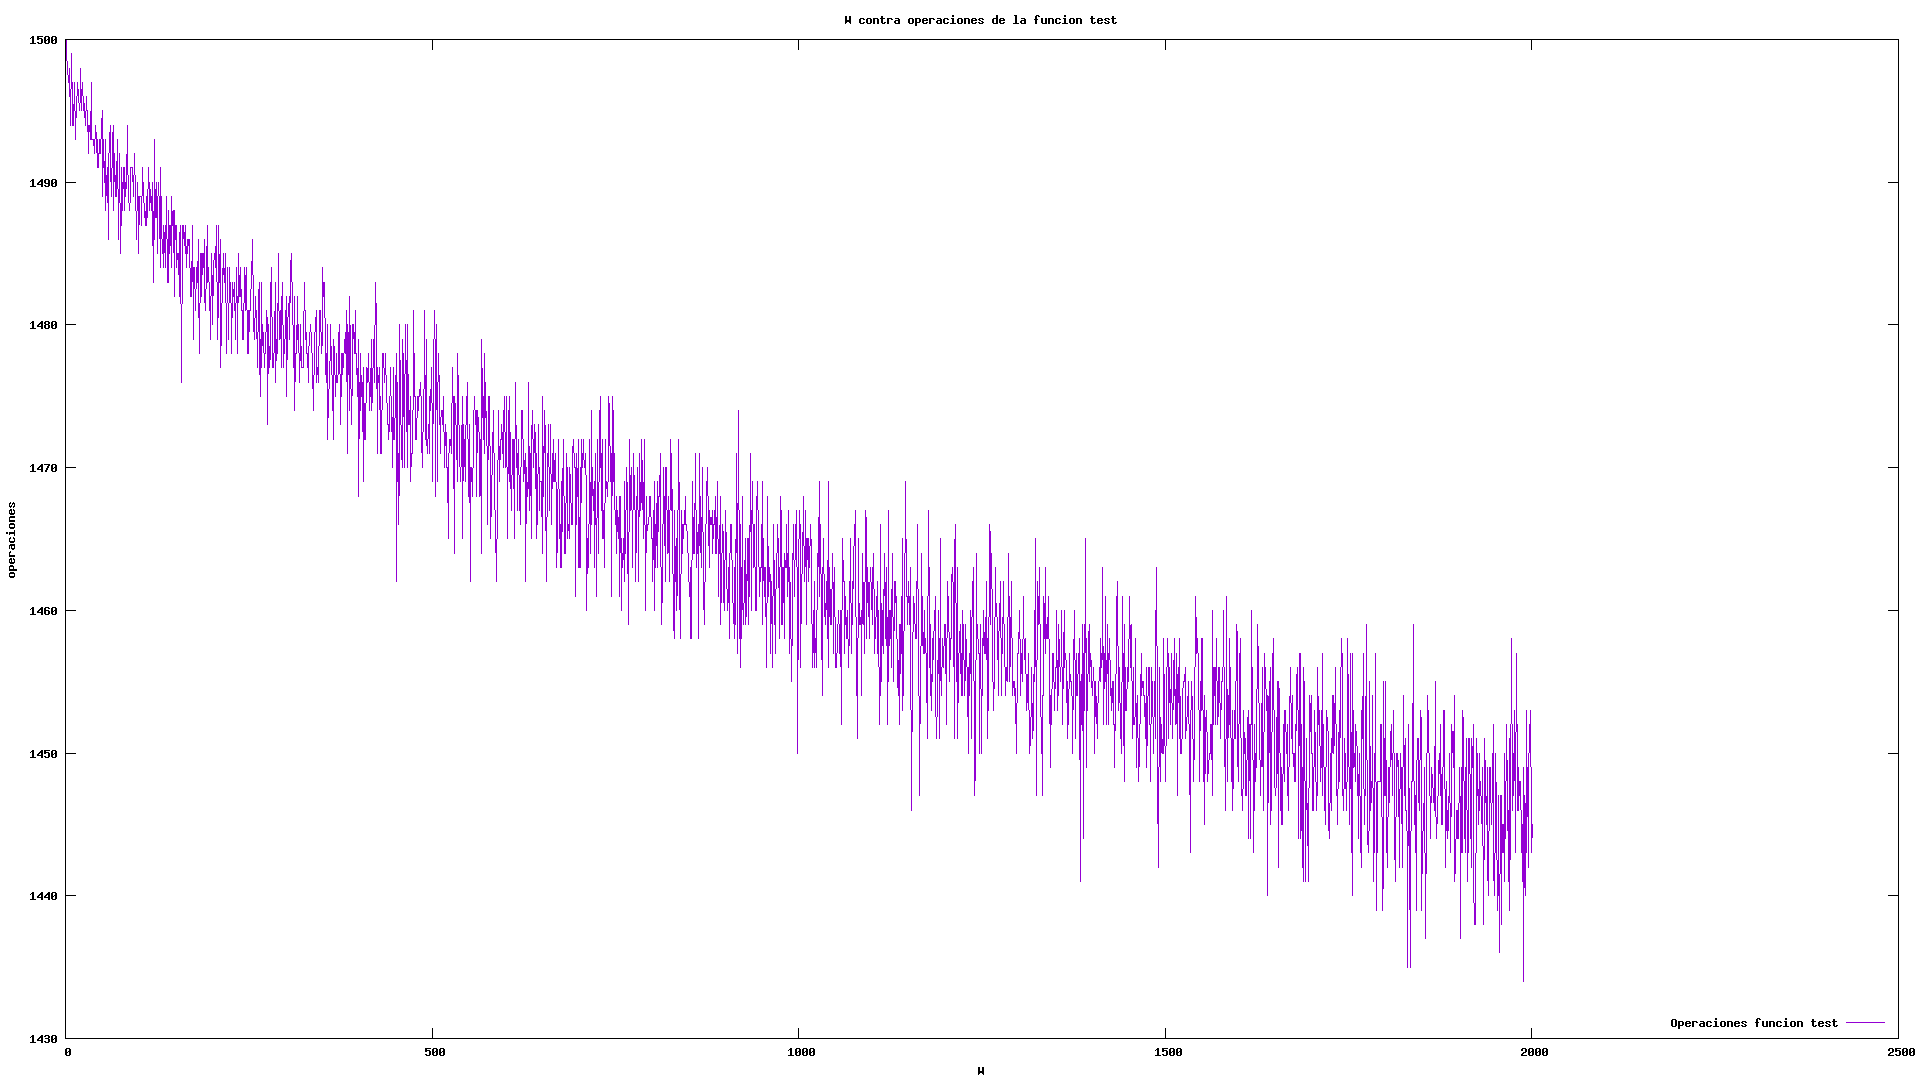
\includegraphics[width=400px,height=300px]{grafica9}
		\caption{W contra operaciones de la funcion test}
	\end{figure}
	\begin{figure}[H]
		\centering
		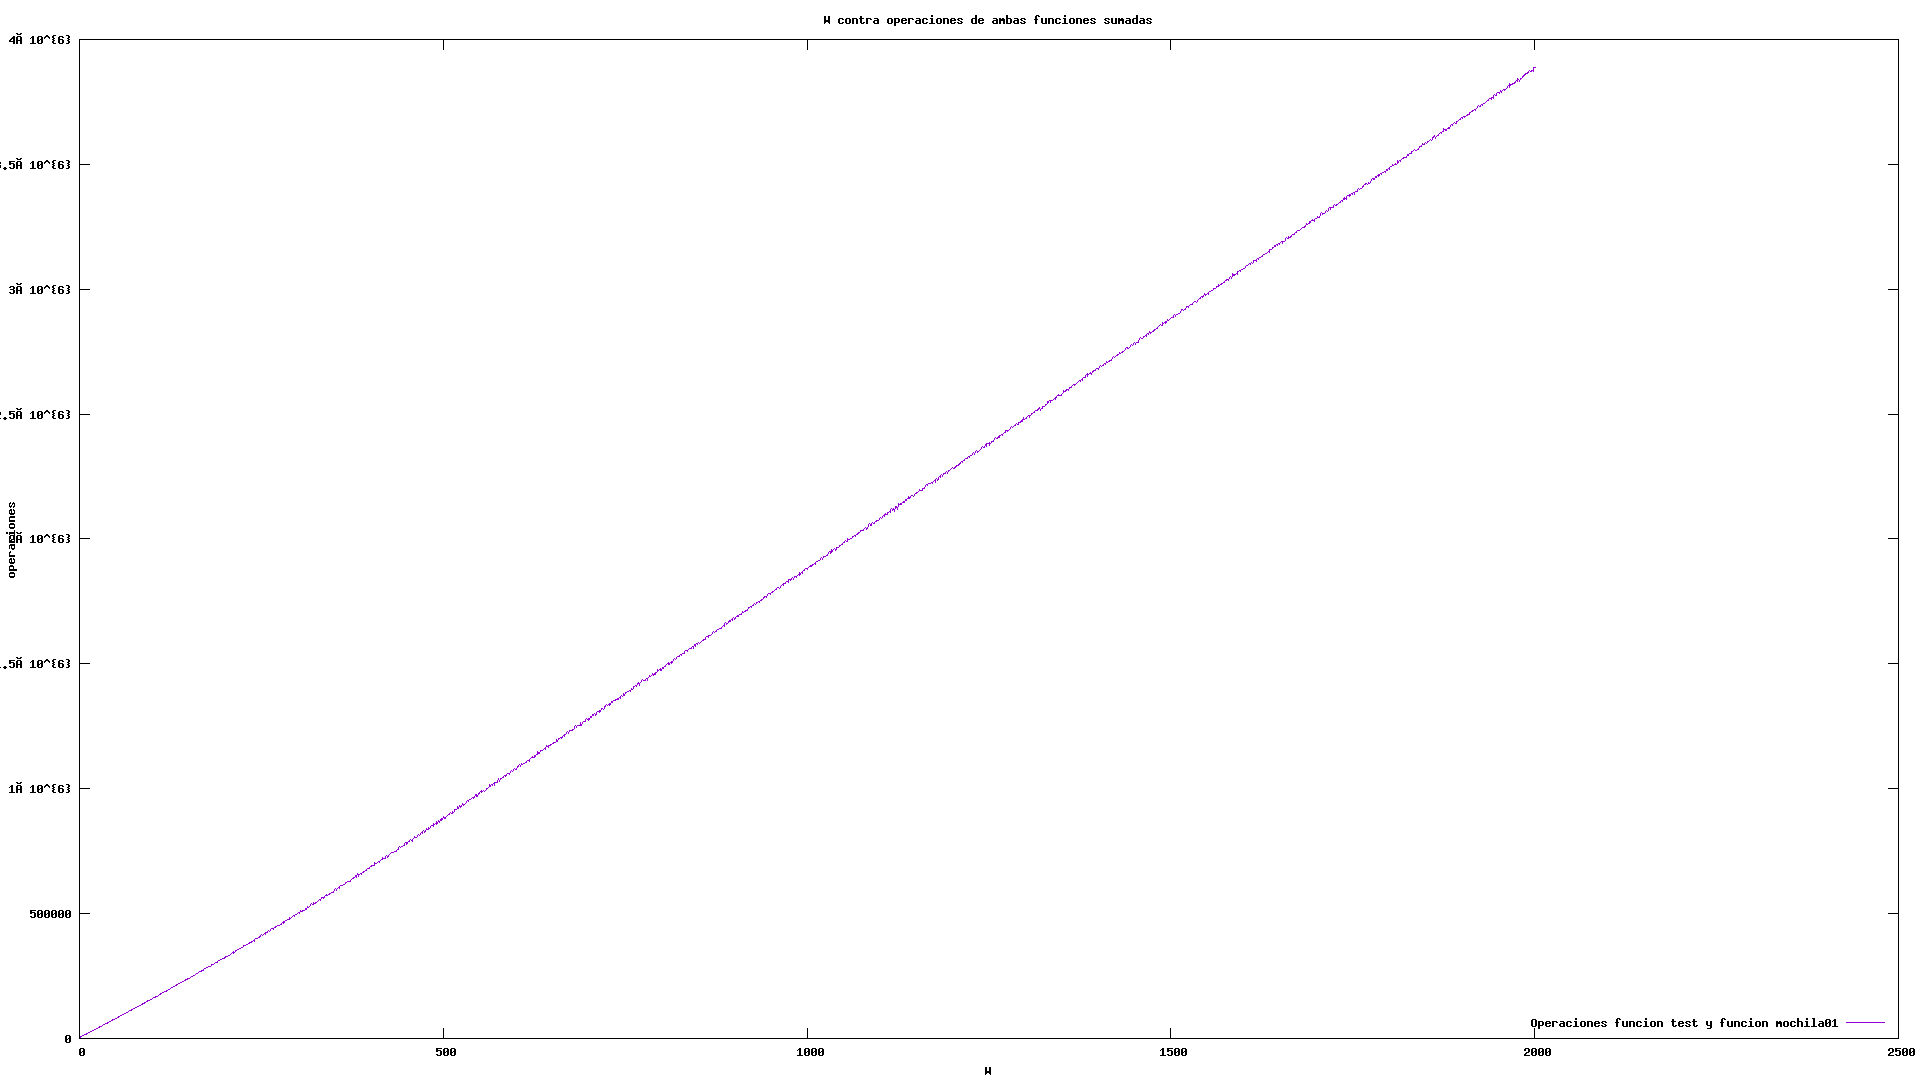
\includegraphics[width=400px,height=300px]{grafica10}
		\caption{W contra operaciones de ambas funciones sumadas}
	\end{figure}
	\begin{figure}[H]
		\centering
		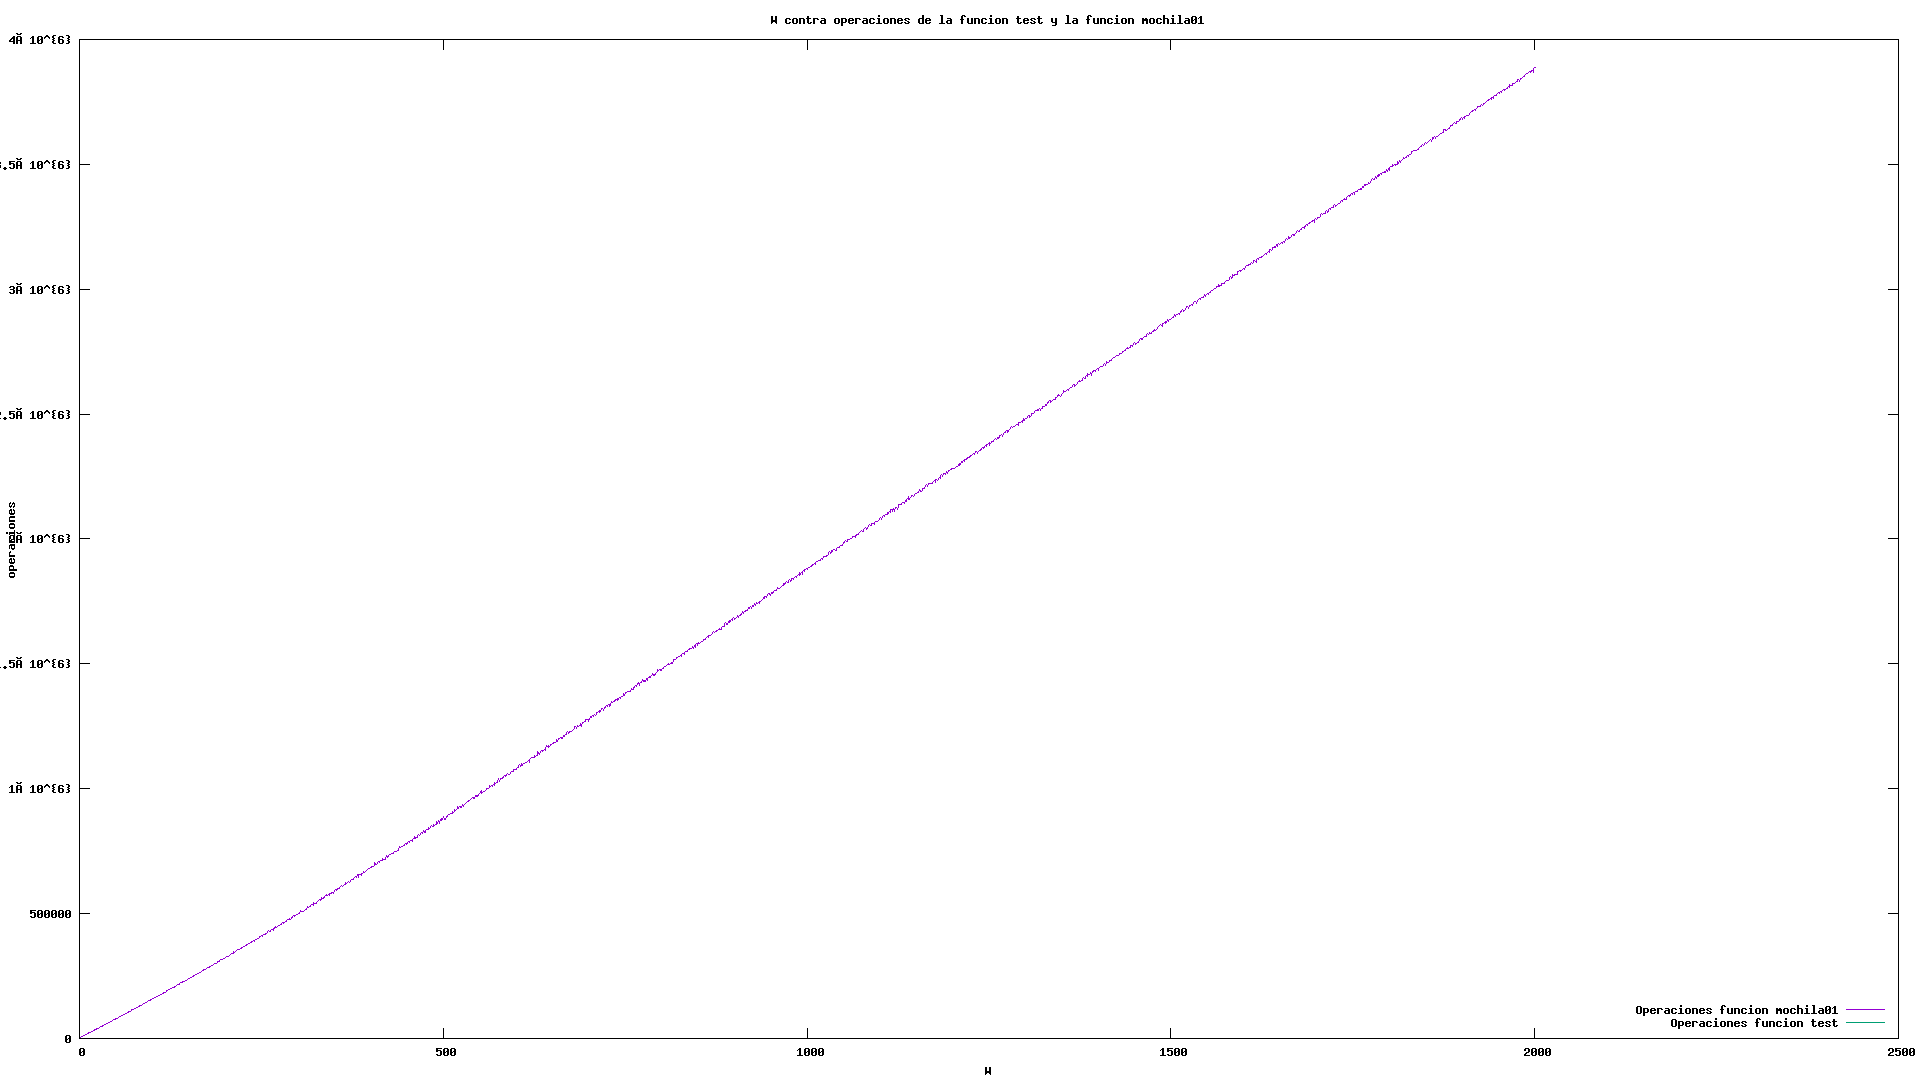
\includegraphics[width=400px,height=300px]{grafica11}
		\caption{W contra operaciones de la funcion test y la funcion mochila01}
	\end{figure}
	Luego se realizaron 5 pruebas controladas de la funcion test, sobre casos especificos y pequeños, uno de ellos el de ejemplo de las clases.\\
	\begin{figure}[H]
		\centering
		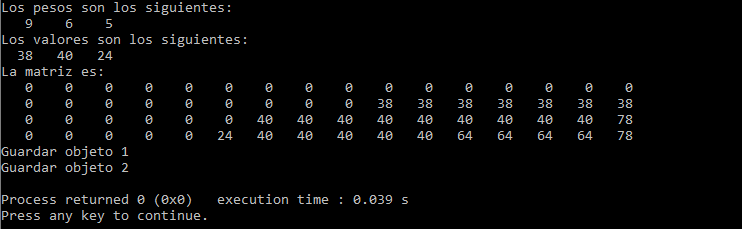
\includegraphics[width=400px,height=300px]{casoEspecifico1}
		\caption{Primer caso especifico probado (El caso de ejemplo del video)}
	\end{figure}
	\begin{figure}[H]
		\centering
		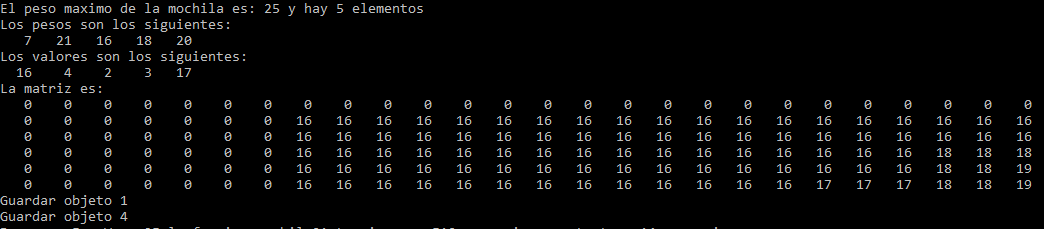
\includegraphics[width=400px,height=300px]{casoEspecifico2}
		\caption{Segundo caso especifico probado}
	\end{figure}
	En este ejemplo (Figure 16), podemos ver que le combiene tomar el primero y cuarto objeto, ya que la suma de pesos es exactamente 25 (la capacidad maxima de la mochila) y la ganancia es de 18, no hay forma de superar esta ya que si tomamos el elemento 5, este no se puede combinar y nos da una ganancia de 17, misma situacion se aplica para todas las demas combinaciones posibles.
	\begin{figure}[H]
		\centering
		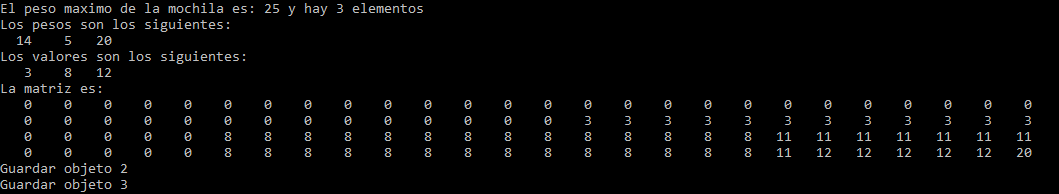
\includegraphics[width=400px,height=300px]{casoEspecifico3}
		\caption{Tercer caso especifico probado}
	\end{figure}
	En este ejemplo (Figure 17), podemos ver que le combiene tomar el segundo y tercer objeto, ya que la suma de pesos es exactamente 25 (la capacidad maxima de la mochila) y la ganancia es de 20, no hay forma de superar esta ya que si tomamos el elemento 1 y lo combinamos con el 2 (el peso queda 19), la ganancia solo es de 15, y no es posible combinar el elemento 1 con el 3.
	\begin{figure}[H]
		\centering
		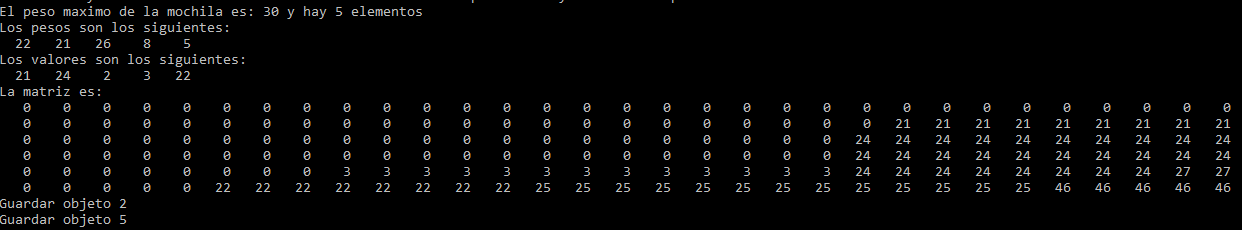
\includegraphics[width=400px,height=300px]{casoEspecifico4}
		\caption{Cuarto caso especifico probado}
	\end{figure}
	En este ejemplo (Figure 18), podemos ver que le combiene tomar el segundo y quinto objeto, ya que la suma de pesos es 26 (4 menos del limite) y la ganancia es de 46, no hay forma de superar esta ya que, todos los valores individuales son menores a 26 y solo se puede combinar el quinto elemento con el primero, segundo (mejor opcion) y cuarto elemento, lo cual da una suma de valores nada equiparable (43, 46 y 45 respectivamente), mientras que al combinar el elemento 4 con el 1 y el 2 obtenemos (24 y 27). Dejando como mejor opcion 2 y 5.
	\begin{figure}[H]
		\centering
		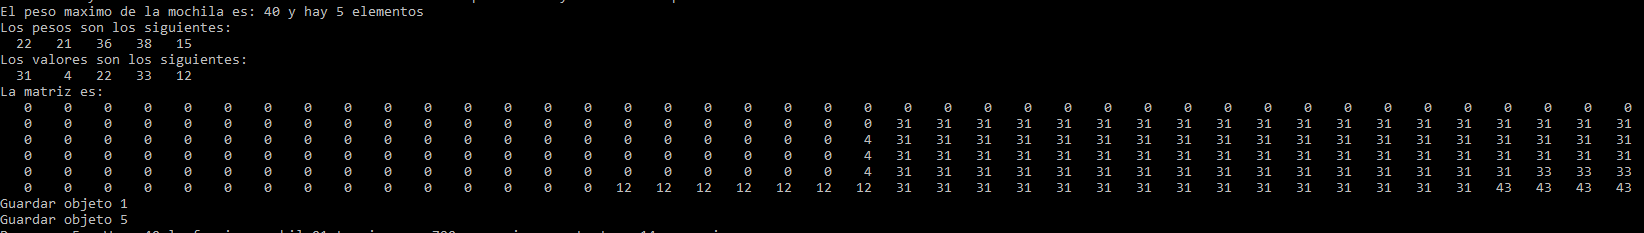
\includegraphics[width=400px,height=300px]{casoEspecifico5}
		\caption{Quinto caso especifico probado}
	\end{figure}
	En este ejemplo (Figure 19), podemos ver que le combiene tomar el primero y quinto objeto, ya que la suma de pesos es 37 (3 por debajo de la maxima capacidad) y la ganancia es de 43, no hay forma de superar esta, ya que los valores individuales de los demas objetos estan por debajo de 43 y solo se pueden combinar 1,2 y 3 de los cuales se obtienen los siguientes valores (35,43,16), finalmente dejando 43 como maximo.\\
	\begin{figure}[H]
		\centering
		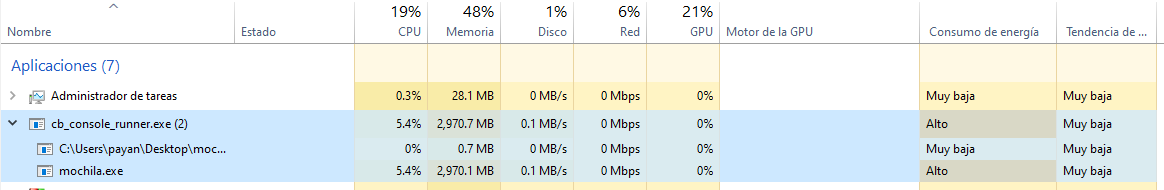
\includegraphics[width=400px,height=150px]{memoria}
		\caption{Memoria RAM durante la ejecucion de los casos a granel}
	\end{figure}
	Como nota adicional, quiero mencionar que el algoritmo consume mucha memoria RAM.\\ 		
	Finalmente se realiza el analisis a priori de la complejidad temporal de ambas funciones y se compararan con los resultados graficados previamente.\\
	Primero el analisis de la funcion mochila01:\\
	\begin{center}
		\begin{table}[H]
			\begin{tabular}{|l|l|l|}
				\hline
				\rowcolor[HTML]{FFCC67} 
				Codigo                           & Costo & Veces ejecutado \\ \hline
				\textit{for(j = 0; j $\leq$ n; j++)}                    & $\O(n)$    & n+2               \\ \hline
				\textit{\  \  retorno[j][0] = 0}                    & $\O(1)$    & n               \\ \hline
				\textit{for(c = 0; c $\leq$ W; c++)}                    & $\O(W)$    & W+2               \\ \hline
				\textit{\  \  retorno[0][c] = 0}                    & $\O(1)$    & W               \\ \hline
				\textit{for(j = 1; j $\leq$ n; j++)}                    & $\O(n*W)$    & n+2               \\ \hline 					
				\textit{\  \  for(c = 1; c $\leq$ W; c++)}                    & $\O(W)$    & n               \\ \hline 
				\textit{\  \  \  \  if(c$<$wt[j-1])}                    & $\O(1)$    & n*W               \\ \hline 
				\textit{\  \  \  \  \  \  retorno[j][c] = retorno[j-1][c]}                    & $\O(1)$    & n*W               \\ \hline 
				\textit{\  \  \  \  else}                    & $\O(1)$    & n*W               \\ \hline 
				\textit{\  \  \  \  \  \  if(retorno[j-1][c] $\geq$ retorno[j-1][c-wt[j-1]]+val[j-1])}                    & $\O(1)$    & n*W               \\ \hline
				\textit{\  \  \  \  \  \  \  \  retorno[j][c] = retorno[j-1][c]}                    & $\O(1)$    & n*W               \\ \hline	
				\textit{\  \  \  \  \  \  else}                    & $\O(1)$    & n*W               \\ \hline
				\textit{\  \  \  \  \  \  \  \  retorno[j][c] = retorno[j-1][c-wt[j-1]]+val[j-1]}                    & $\O(1)$    & n*W               \\ \hline							
				\textit{return retorno}                    & $O(1)$    & 1               \\ \hline 				
			\end{tabular}
		\end{table}										
	\end{center}
	Como podemos observar y apoyados por las graficas (Figure 11 y Figure 6) la complejidad de esta funcion esta marcada por el los dos for anidados que la vuelven $\O(n*W)$, es decir que depende tanto del peso maximo de la mochila, como de la cantidad maxima de objetos a guardar. Puede interpretarse como lineal sobre n, siempre y cuando W sea discriminable, en cualquier otro caso no.\\
	Ahora se analiza la complejidad temporal de la funcion test\\
	\begin{center}
		\begin{table}[H]
			\begin{tabular}{|l|l|l|}
				\hline
				\rowcolor[HTML]{FFCC67} 
				Codigo                           & Costo & Veces ejecutado \\ \hline
				\textit{if(j$>$0)}                    & $\O(n)$    & 1               \\ \hline
				\textit{\  \  if(c $<$ wt[j-1])}                    & $\O(1)$    & 1               \\ \hline
				\textit{\  \  \  \  test(j-1,c,val,wt,matriz,contador)}                    & $T(n-1))$    & 1               \\ \hline
				\textit{\  \  else}                    & $\O(1)$    & 1               \\ \hline
				\textit{\  \  \  \  if(matriz[j-1][c-wt[j-1]]+val[j-1]$>$matriz[j-1][c])}                    & $\O(1)$    & 1               \\ \hline 					
				\textit{\  \  \  \  \  \  test(j-1,c-wt[j-1],val,wt,matriz,contador)}                    & $T(n-1)$    & 1               \\ \hline
				\textit{\  \  \  \  \  \  print("Guardar objeto ",j)}                    & $O(1)$    & 1               \\ \hline  
				\textit{\  \  \  \  else}                    & $\O(1)$    & 1              \\ \hline 
				\textit{\  \  \  \  \  \  test(j-1,c,val,wt,matriz,contador)}                    & $T(n-1)$    & 1               \\ \hline 								
			\end{tabular}
		\end{table}										
	\end{center}
	Cuando terminamos el analisis de la funcion nos queda la siguiente ecuacion de recurrencia $T(x) = T(x-1) + C$ donde $x = n*W$, esta ya es una ecuacion conocida, que al resolverla nos queda que $T(x) = Cx$ asi que al final $T(x)=\O(n*m)$, cosa que podemos comprobar en las graficas (Figure 12 y Figure 7), donde se aprecia que en ambos acercamientos (iterando n o iterando W), crece de forma lineal, lo cual indica que depende de ambas variables para crecer. Se asume que $x = n*W$ ya que el espacio de busqueda es la matriz que obtenemos de la funcion "mochila01", y como podemos observar si se reduce uno u otro de los indices sigue siendo el mismo espacio de busqueda.
	\section{Conclusiones}			
	\subsection{Payán Téllez René}
	Esta practica fue particularmente larga ya que aunque implementar los algoritmos fue algo sencillo, el desarrollar todo lo que necesitaban para poder ser probados no lo fue, sin mencionar que calcular la complejidad de ambos es complicado, aunque son ecuaciones de recurrencia que se han visto en clase, el encontrar la forma de que los datos crudos, las graficas y los calculos a priori tengan sentido no lo es tanto. Inclusive el realizar la parte experimental tuvo sus inconvenientes, por ejemplo en la secuencia de fibonacci se desbordaban los enteros, asi que se tuvieron que reemplazar por long long int, y en la mochila, esta consumia una cantidad enorme de memoria ram, hasta llego a detener la computadora por completo. Pero aun asi puedo decir que aprendi al menos los inicios de un tema muy complicado y util que es la programacion dinamica.\\
	\includegraphics[height=120px,width=120px]{Rene}
	\section{Anexo}			
	\section{Bibliografia}
	{[}1{]}\url{http://www.lcc.uma.es/~av/Libro/CAP3.pdf}\\
	{[}2{]}\url{https://medium.com/@joseguillermo_/qu\%C3\%A9-es-la-complejidad-algor\%C3\%ADtmica-y-con-qu\%C3\%A9-se-come-2638e7fd9e8c}\\
	{[}3{]}\url{https://www.tamps.cinvestav.mx/~ertello/algorithms/sesion15.pdf	}\\		
	{[}4{]}\url{http://elvex.ugr.es/decsai/algorithms/slides/4\%20greedy.pdf}\\			
	{[}5{]}\url{http://cms.dm.uba.ar/materias/1ercuat2009/optimizacion/Maurette_Ojea.pdf}\\
	{[}5{]}\url{https://riptutorial.com/es/algorithm/example/23995/codificacion-huffman}\\	
	{[}6{]}\url{https://quantdare.com/numeros-de-fibonacci/}\\	
	{[}7{]}\url{https://www.geeksforgeeks.org/0-1-knapsack-problem-dp-10/}\\			
\end{document}